\documentclass{beamer}

\usetheme{Berlin}
\definecolor{arduino}{rgb}{0.0, 0.6, 0.61}
\definecolor{scarlet}{rgb}{1.0, 0.13, 0.0}
\definecolor{darkviolet}{rgb}{0.58, 0.0, 0.53}
\definecolor{raspberry}{rgb}{0.89, 0.04, 0.36}
\usecolortheme[named = darkviolet]{structure}


\title[Programación Avanzada]{Programación Avanzada}
\subtitle{Sesión 8: Introducción a Arduino}
\author{Víctor de Jesús Medrano Zarazúa \\
	\textit{vdejesusmedrano@gmail.com}\\}
\institute{Universidad del Valle de México}
\date{9 de octubre de 2017}

\usepackage[spanish]{babel}
\usepackage[T1]{fontenc}
\usepackage{multicol}
\usepackage{alltt}
\usepackage{verbatim}
\usepackage{xcolor}
\usepackage{caption}
\usepackage{animate}
\usepackage{media9}
\setbeamertemplate{caption}[numbered]

\begin{document}
	
	\begin{frame}
		\titlepage
	\end{frame}
	
	\begin{frame}[t]{Contenido}\vspace{4pt}
		%\begin{multicols}{2}
		\tableofcontents
		%\end{multicols}
	\end{frame}
	
	\begin{frame}
		\textit{"Technology shouldn't facilitate you feeling like garbage. Use technology to transcend your shitty confines.
			It's not your fault (not all the time, anyway). Realize that, and for crying out loud, don't be technology's bitch. Make technology your bitch."}\\
		\textcolor{magenta}{\textbf{Maynar O' Lion}}
	\end{frame}
	
	\section{Introducción}
	\begin{frame}{?`Qué es Arduino?}
		Simple placa de entrada salida (E/S) y un entorno de desarrollo (IDE).
		
		\begin{multicols}{2}
			\begin{figure}
				\label{fig:ard}
				\centering
				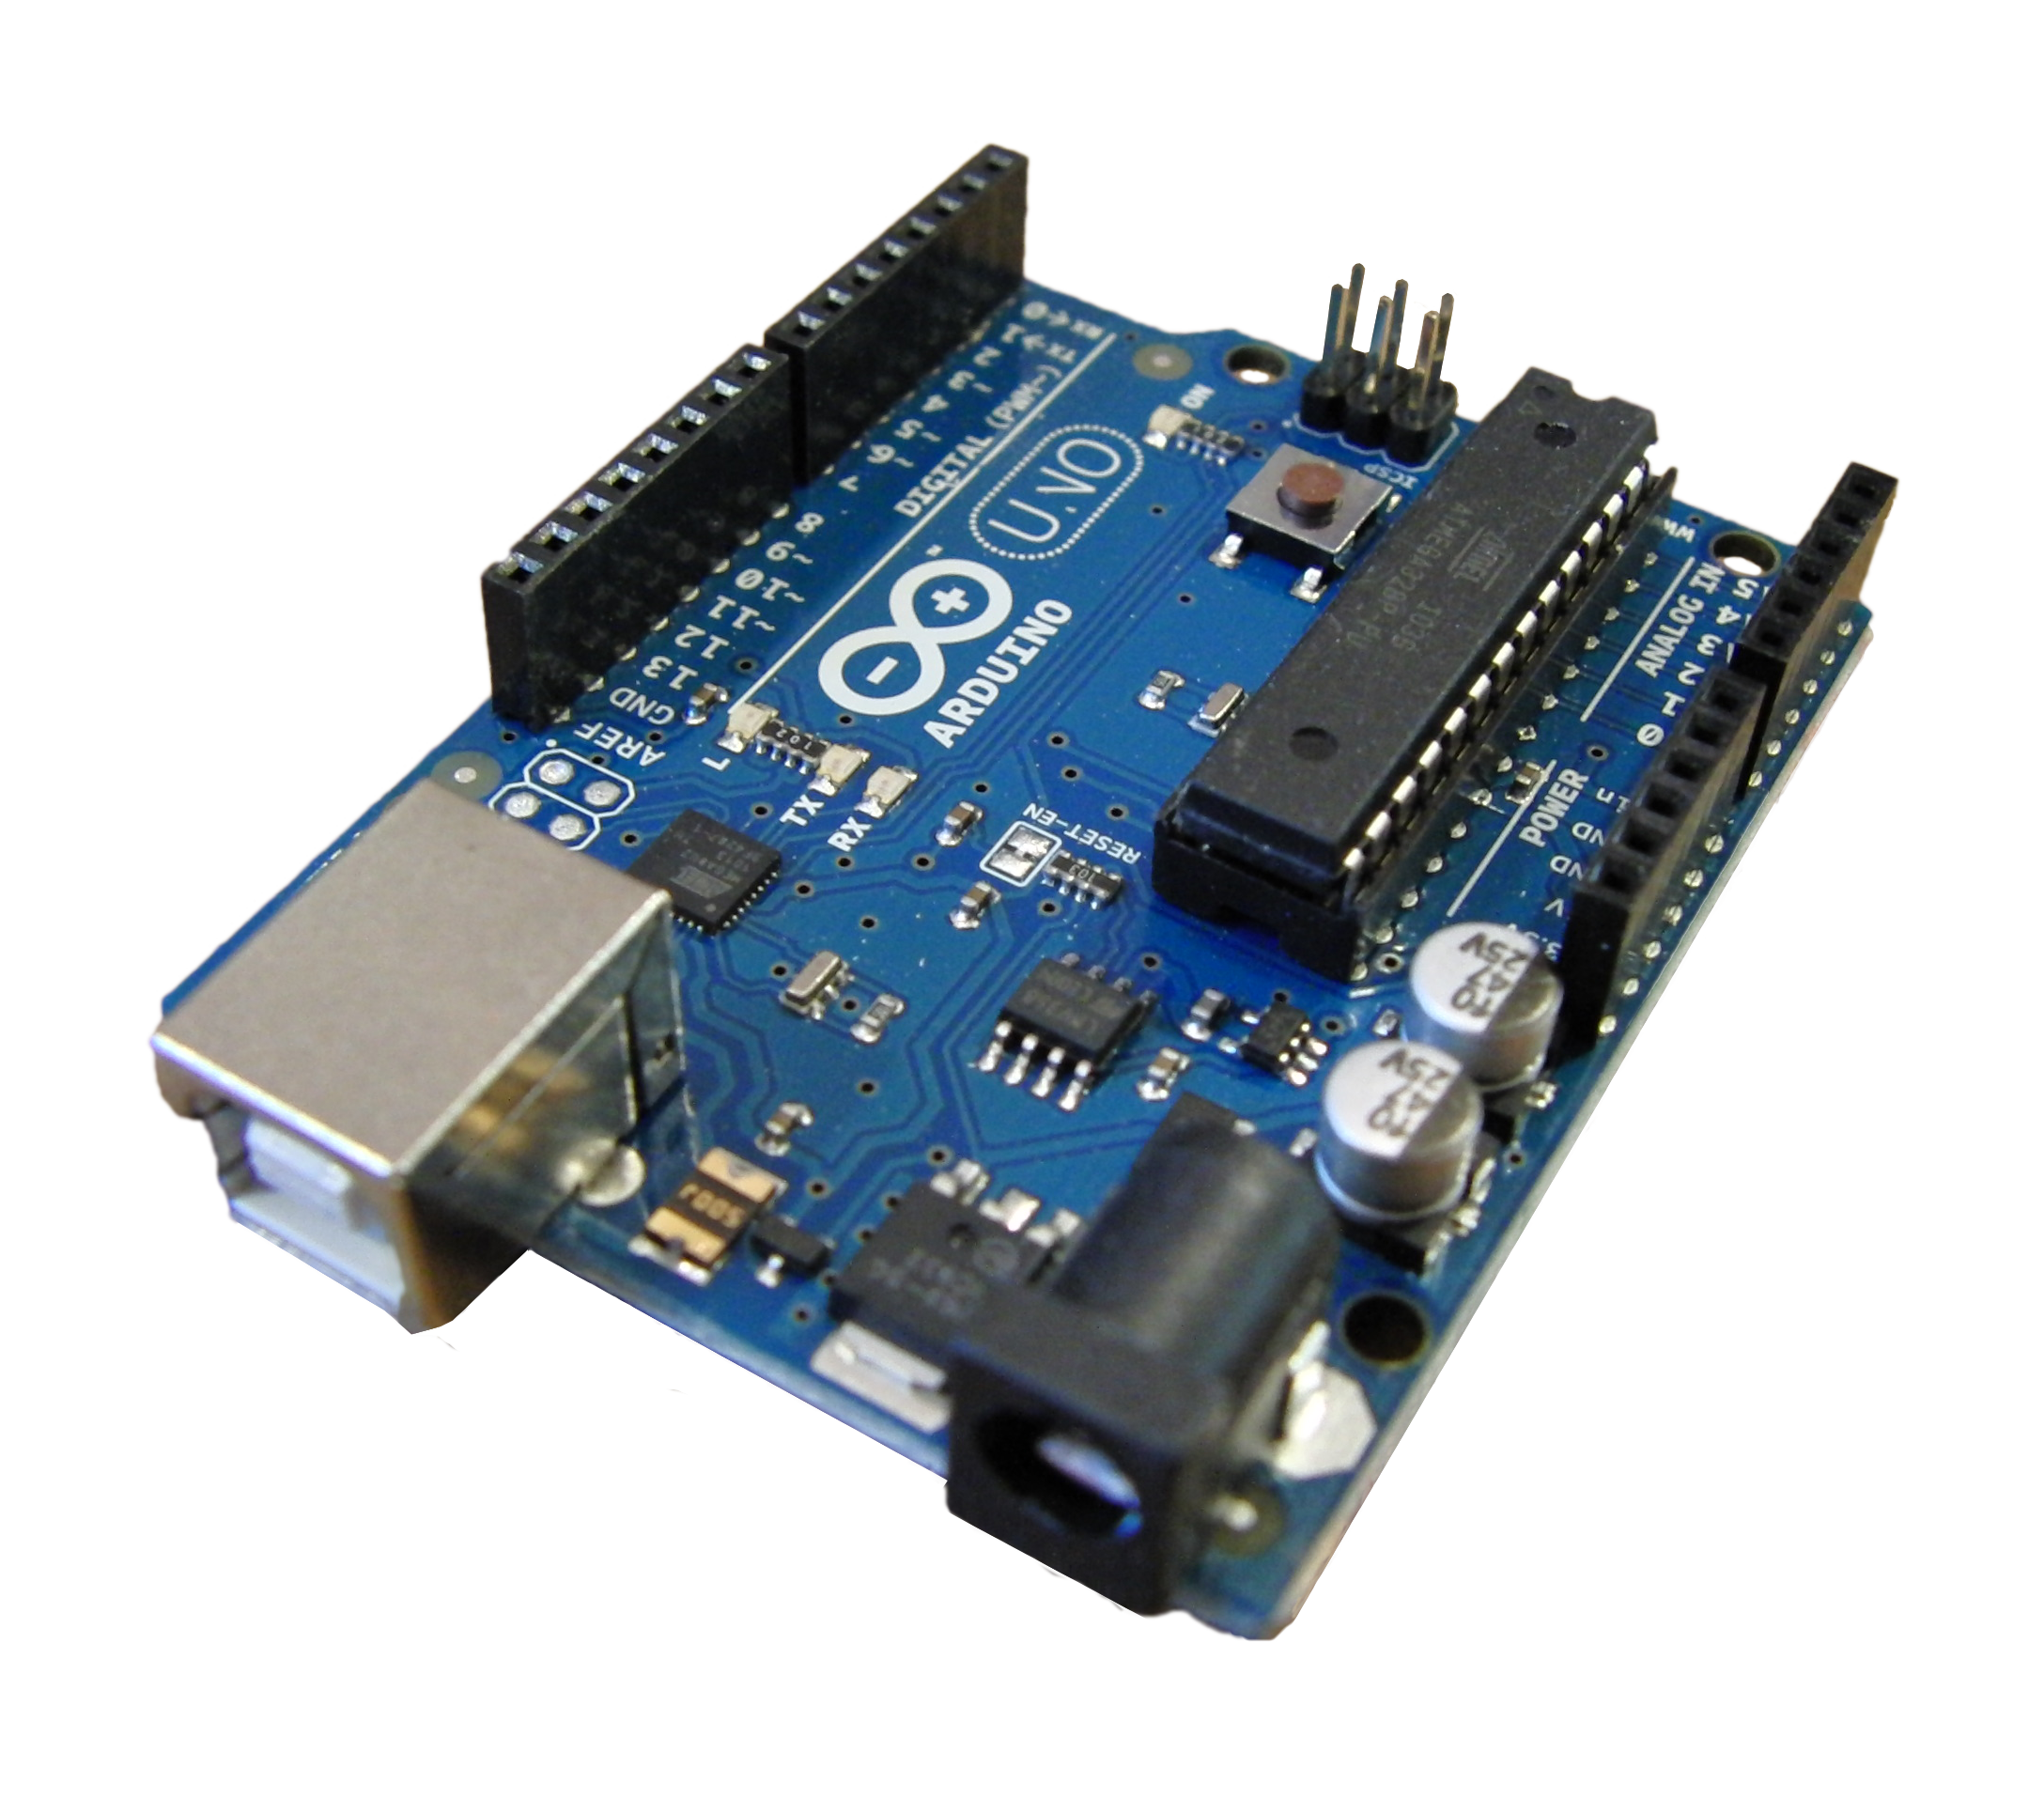
\includegraphics[scale=0.05]{arduino}
				\caption{Sistema Embebido}
			\end{figure}
			\begin{figure}
				\label{fig:ide}
				\centering
				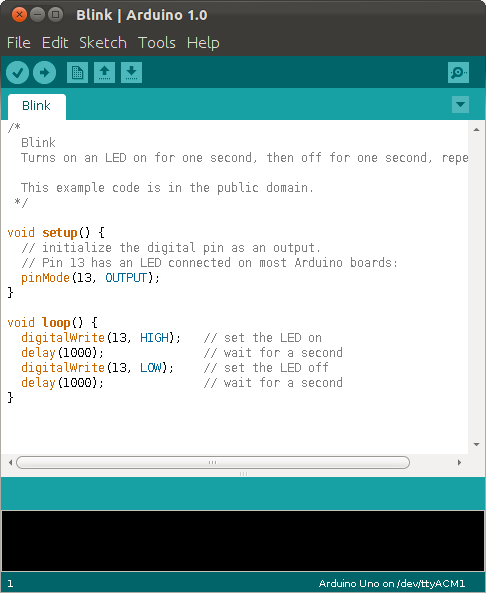
\includegraphics[scale=0.2]{ide}
				\caption{Integrated Development Environment (IDE)}
			\end{figure}
		\end{multicols}
	\end{frame}
	
	\begin{frame}{?`Por qué Arduino?}
		\begin{itemize}
			\item Multiplataforma (Linux, Windows, macOS, etc.)
			\item Entorno de programación simple y claro (basado en Processing)
			\item Código abierto (Hardware/Software Extensible)
			\item Económico
			\item Comunidad de usuarios activa
			\item Didáctico
		\end{itemize}
	\end{frame}
	
	\begin{frame}{Computación física}
		Interacción entorno-objeto por medio sensores y actuadores controlados por un software dentro de un chip.
		\begin{figure}
			\centering
			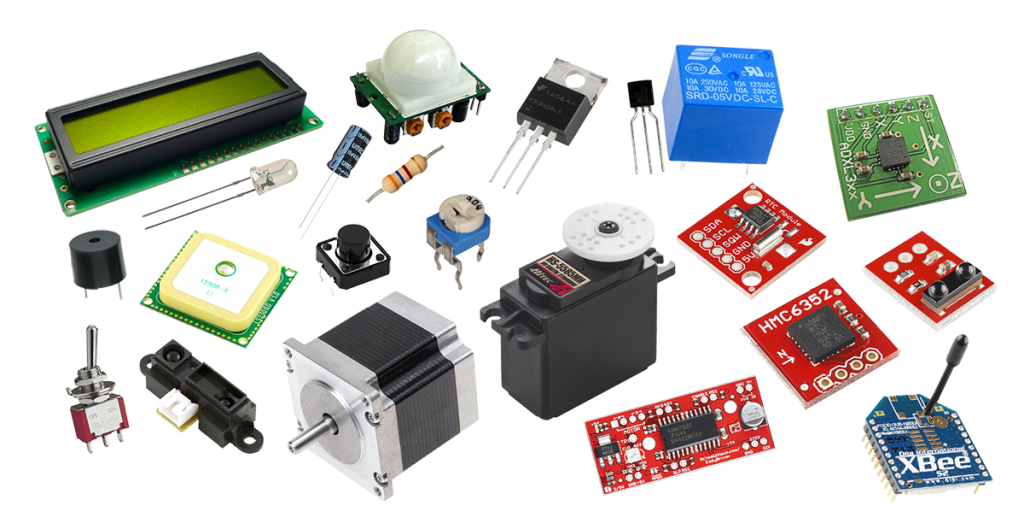
\includegraphics[scale=0.25]{senact}
		\end{figure}
	\end{frame}
	
	\section{Filosofía de Arduino}
		\begin{frame}{Tinkering}
			Explorar el medio de una forma abierta y encontrar lo inesperado (experimentar).
			\begin{multicols}{2}
				\begin{figure}
					\centering
					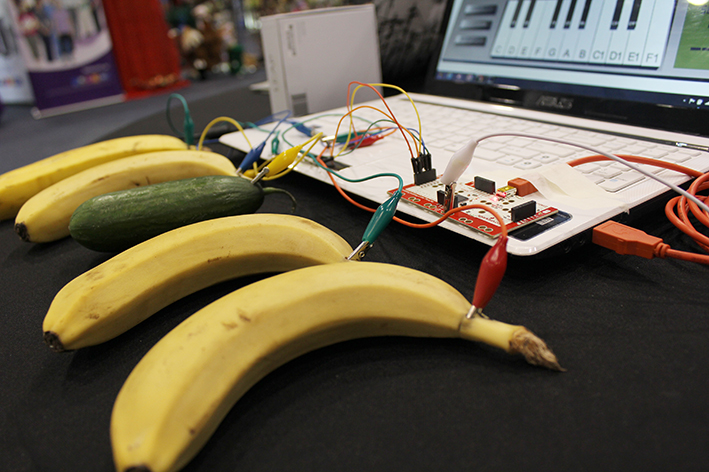
\includegraphics[scale=0.22]{tink1}
				\end{figure}
				\begin{figure}
					\centering
					
\includegraphics[scale=0.19]{tink2}
				\end{figure}
			\end{multicols}
			
		\end{frame}
		\begin{frame}{Parchar}
			Capacidad de crear sistemas complejos mediante la unión de dispositivos simples (e.g., Sintetizadores Moog).\vspace{0.5cm}
			
			\centering
			\animategraphics[autoplay,loop, width = \linewidth, scale = 0.7]{12}{moog-}{0}{23}
	
		\end{frame}
		
%		\begin{frame}{On The Run}
%			
%			\includemedia[
%			width=0.4\linewidth,
%			totalheight=0.225\linewidth,
%			activate=pageopen
%			]{\fbox{Click!}}{https://www.youtube.com/watch?v=VouHPeO4Gls}
%			
%		\end{frame}
		
		\begin{frame}{Circuit bending}
			Es la modificación creativa de dispositivos de audio electrónicos activados por pilas.
			\begin{figure}
				\centering
				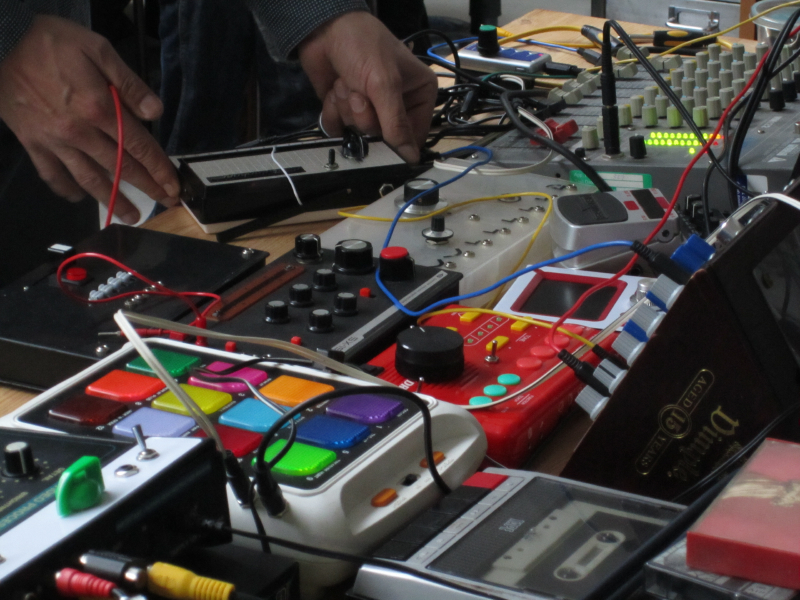
\includegraphics[scale=0.25]{bending}
			\end{figure}
		\end{frame}				
		\begin{frame}{Reciclar}
			\begin{figure}
				\centering
				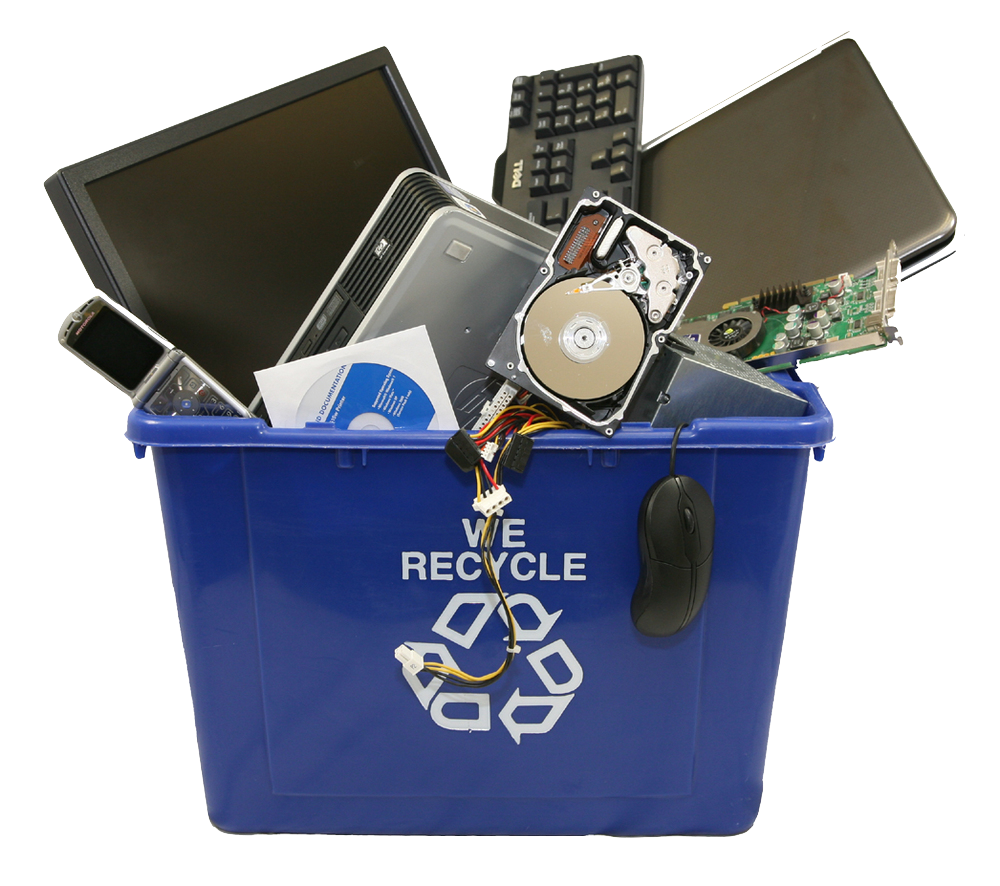
\includegraphics[scale=0.2]{recycle}
			\end{figure}
		\end{frame}	
		\begin{frame}{Colaborar}
			\begin{figure}
				\centering
				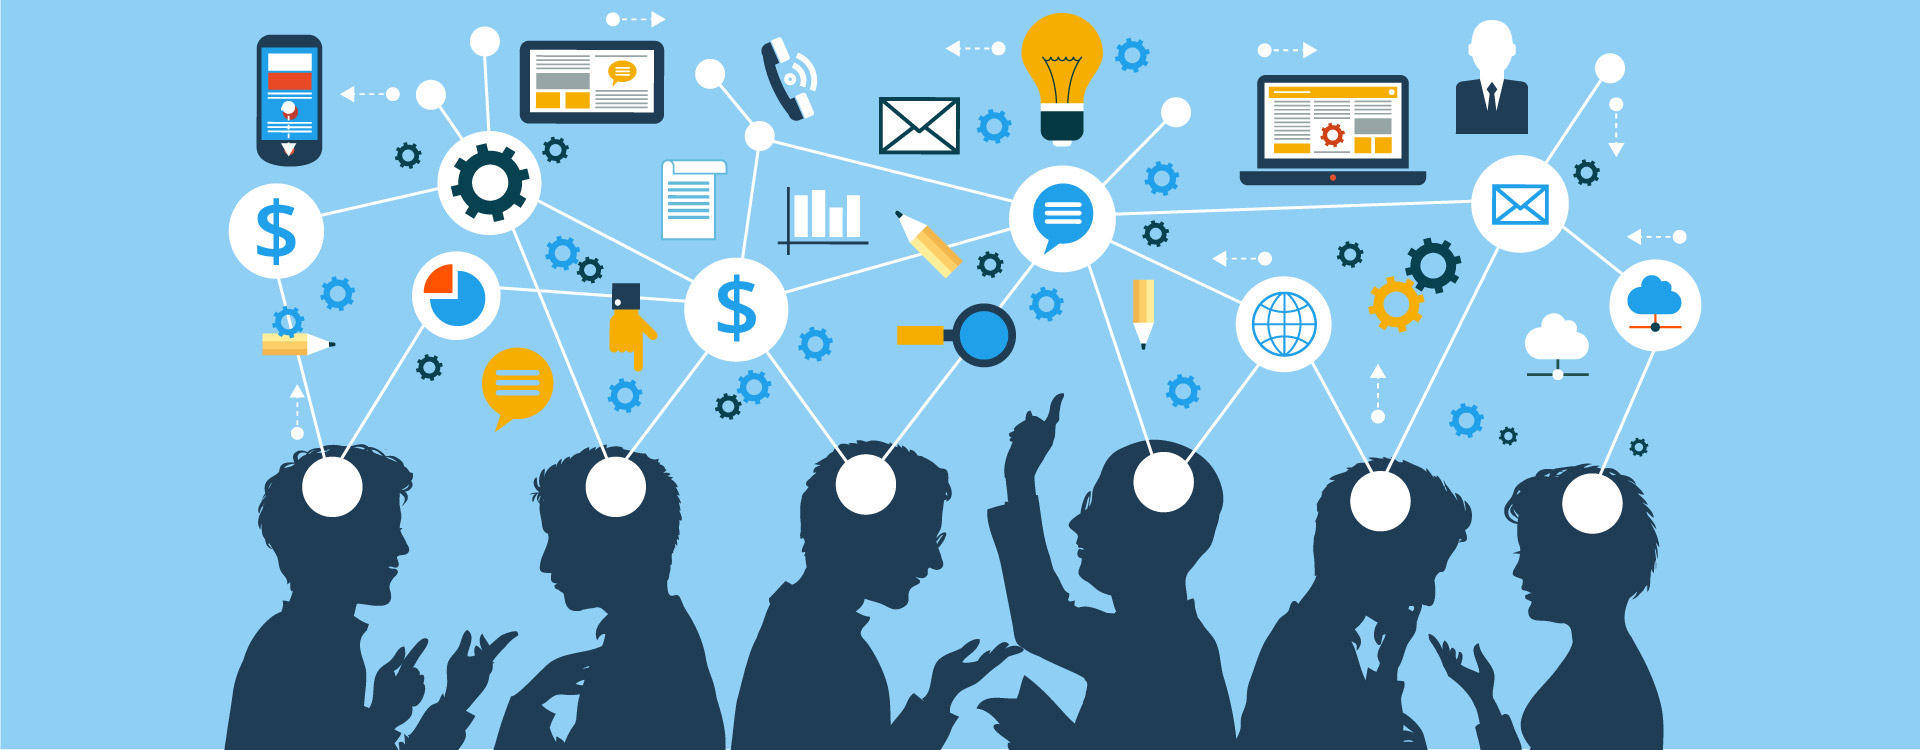
\includegraphics[width=\linewidth]{collaboration}
			\end{figure}
			
		\end{frame}	
		
		\begin{frame}{Colaborar}
			\begin{block}{Código abierto}
				Cuando los programadores (en Internet) pueden \textcolor{raspberry}{leer, modificar y redistribuir} el código fuente de un programa, este evoluciona, se desarrolla y mejora.
			\end{block}
		\end{frame}		
	
	\section{Plataforma de Arduino}
	
	\begin{frame}{Placa de Arduino (Hardware)}
		\begin{figure}
			\centering
			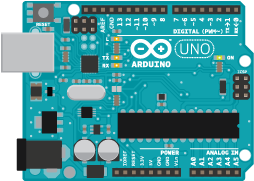
\includegraphics[scale=0.55]{ardu}
		\end{figure}
	\end{frame}
	
	\begin{frame}{Partes del hardware}
		\begin{figure}
			\centering
			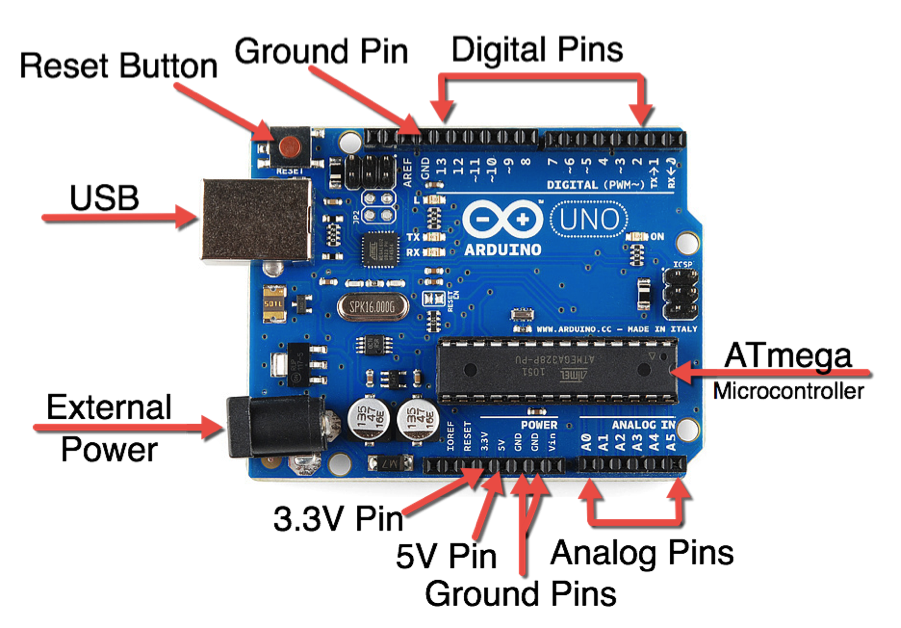
\includegraphics[scale=0.55]{arduinoparts}
		\end{figure}
	\end{frame}
	
	\begin{frame}{Entorno de programación (Software)}
		\begin{figure}
			\centering
			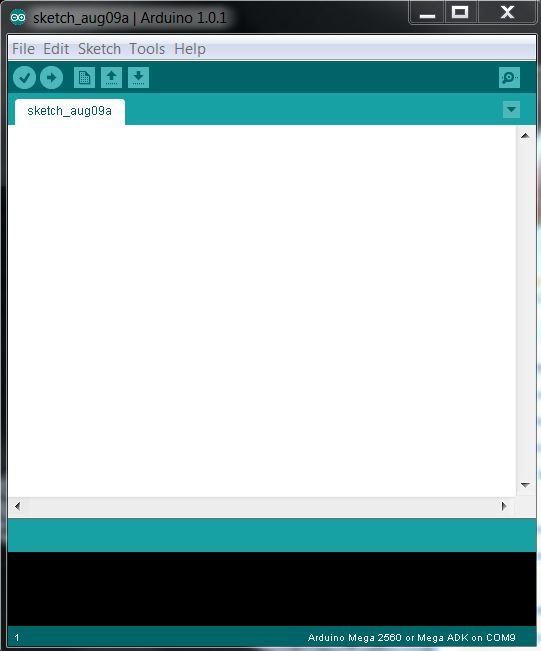
\includegraphics[scale = 0.45]{ide2}
		\end{figure}
	\end{frame}
	
	\begin{frame}{Partes del IDE}
		\begin{figure}
			\centering
			\def\svgwidth{\columnwidth}
			\input{partside.pdf_tex}
		\end{figure}
	\end{frame}
	
	\begin{frame}{Comunicación en Sistemas Embebidos}
		\begin{multicols}{3}
			\begin{figure}
				\centering
				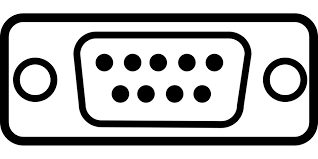
\includegraphics[scale=0.31]{serial}
				%\caption{Desarrollo de software}
			\end{figure}
			\begin{figure}
				\centering
				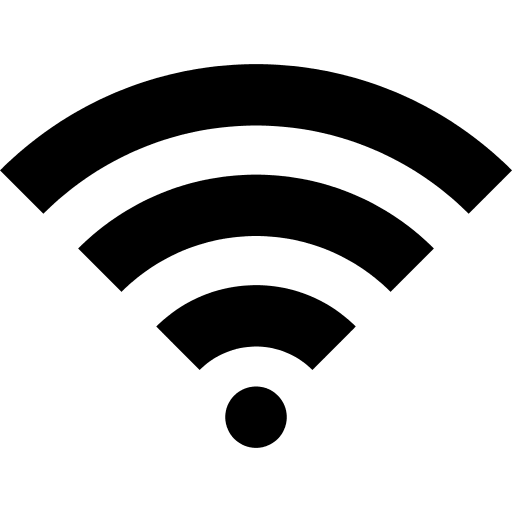
\includegraphics[scale=0.2]{wifi}
				%\caption{Análisis numérico}	
			\end{figure}
			\begin{figure}
				\centering
				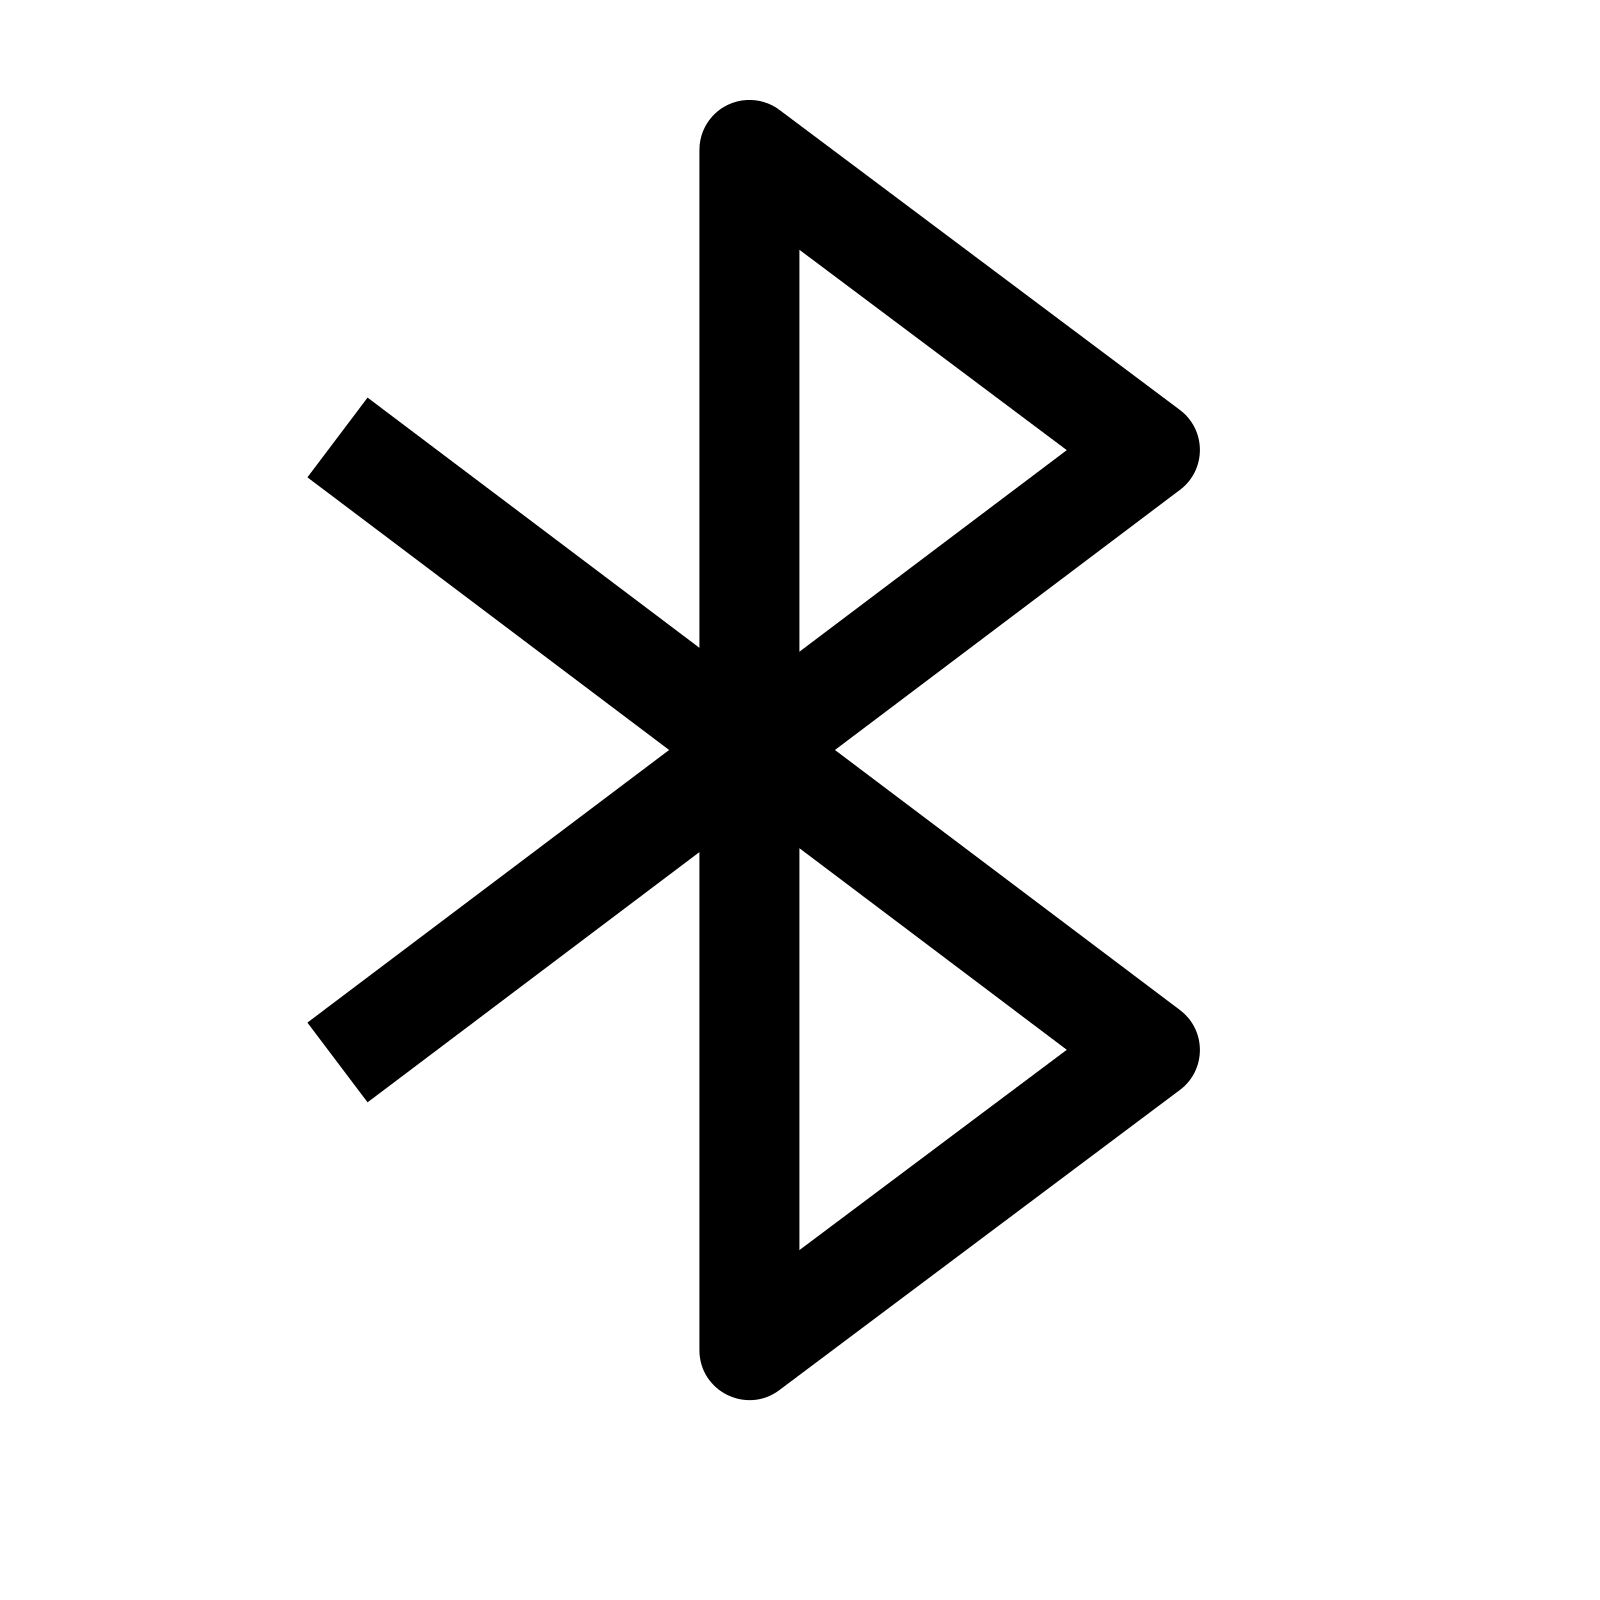
\includegraphics[scale=5.4]{bluetooth}
				%\caption{Multimedia}
			\end{figure}
		\end{multicols}
	\end{frame}
	
	\begin{frame}{Creador: Massimo Banzi}
		\begin{figure}
			\centering
			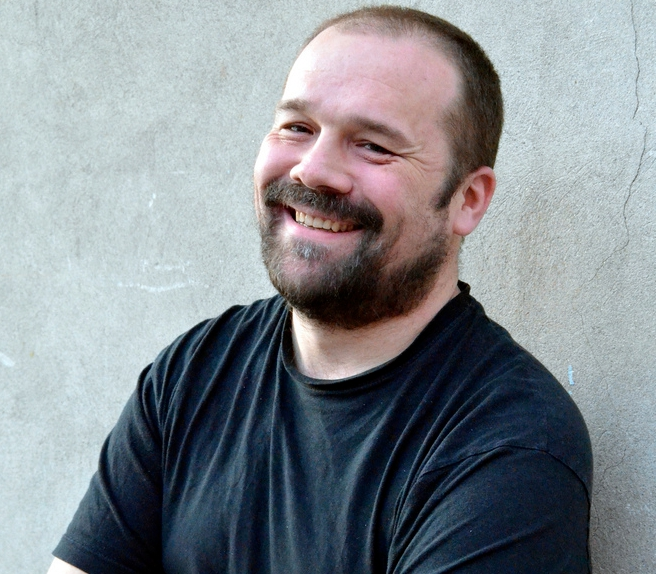
\includegraphics[scale=0.25]{banzi}
			\caption{Santo patrono de Arduino}
		\end{figure}
	\end{frame}
	
\end{document}